\documentclass[a4paper]{article}
\usepackage[utf8]{inputenc}
\usepackage{graphicx} 
\usepackage[margin=1 in]{geometry}
\usepackage{fancyhdr}
\pagestyle{fancy}
\usepackage[dvipsnames]{xcolor}
\usepackage{hyperref}
\usepackage{secdot}

%Abdullah Al Zobayer

\lhead{
\tiny
Indian Journal of Science and Technology, Vol 9(38), DOI: 10.17485/ijst/2016/v9i38/102967, October 2016}

\rhead{
\small
ISSN (Print) : 0974-6846\\ ISSN (Online) : 0974-5645}

\lfoot{
\tiny
Vol 9 (38) | October 2016 | \href{https://www.indjst.org/}{www.indjst.org}
}
\rfoot{
\tiny
Indian Journal of Science and Technology
}



\begin{document}


\begin{flushright}
\huge
\textcolor{BlueViolet}
{\textbf{Text to Speech Conversion}}\\
\vspace{3mm} 
\large
S. Venkateswarlu \textsuperscript{1*}, D. B. K. Kamesh \textsuperscript{1}, J. K. R. Sastry \textsuperscript{2} and Radhika Rani \textsuperscript{2}

\small
\textsuperscript{1}Department of CSE, K L University, Vaddeswarm, Guntur – 522502, Andhra Pradesh, India\;\\

somu23@kluniversity.in,kameshdbk\@kluniversity\.in\, radhikarani\_cse\@kluniversity\.in \\

\textsuperscript{2}Department of ECM, K L University, Vaddeswarm, Guntur – 522502, Andhra Pradesh, India;\\
drsastry@kluniversity.in

\end{flushright}
\hrule

\large
\vspace{5mm}
\begin{flushleft}
\textcolor{BlueViolet}
{\textbf{Abstract}}\\
\end{flushleft}
\small
The present paper has introduced an innovative, efficient and real-time cost beneficial technique that enables user to hear the contents of text images instead of reading through them. It combines the concept of Optical Character Recognition (OCR) and Text to Speech Synthesizer (TTS) in Raspberry pi. This kind of system helps visually impaired people to interact with computers effectively through vocal interface. Text Extraction from color images is a challenging task in computer vision. Text-to-Speech conversion is a method that scans and reads English alphabets and numbers that are in the image using OCR technique and changing it to voices. This paper describes the design, implementation and experimental results of the device. This device consists of two modules, image processing module and voice processing module. The device was developed based on Raspberry Pi v2 with 900 MHz processor speed.

\vspace{5mm}
\large
\textcolor{BlueViolet}
{Keywords:}
\small
Image Processing, OCR, Text Extraction, Text-to-speech, Voice Processing

\textcolor{BlueViolet}
{\section{Introduction}}
\small
Optical character Recognition (OCR) is a process that converts scanned or printed text images1, handwritten text into editable text for further processing. This paper has presented a robust approach for text extraction and converting it to speech. Testing of device was done on raspberry pi platform. The Raspy is initially connected to the internet through VLAN. The software is installed using command lines. Following steps are to be followed:

\begin{enumerate}
    \item The first setup is to download the installation script,
    \item Second step is to convert it to executable form and
    \item The last step starts the script which does the rest of the installation work.
\end{enumerate}
Device set up is done as shown in Figure 1. The web- cam is manually focused towards the text. Then, it takes a picture; a delay of around 7 seconds is provided, which helps to focus the webcam, if it is accidently defocused.After delay, picture is taken and processed by Raspy to hear the spoken words of the text through the earphone or speaker plugged into Raspy through its audio jack.

\vspace{5mm}
\begin{figure}[h]
    \centering
    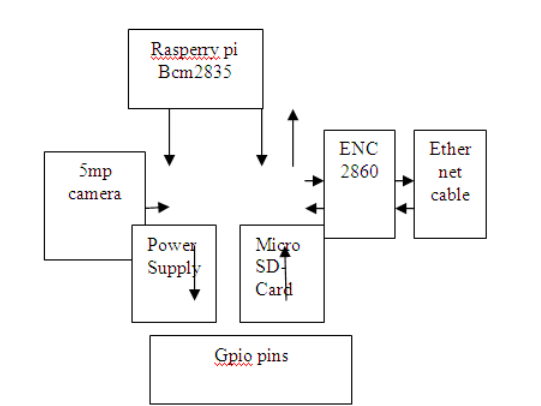
\includegraphics[scale = 0.8]{img1.png}
    \caption{Block diagram of text to speech conversion.}
    \label{fig:enter-label}
\end{figure}

\textcolor{BlueViolet}
{\section{Methodology}}
\small
Text-to-speech device consists of two main modules, the image processing module and voice processing modules.Image processing module captures image using camera, converting the image into text. Voice processing mod- ule changes the text into sound and processes it with specific physical characteristics so that the sound can be understood. Figure 2 shows the block diagram of Text- To-Speech device, 1st block is image processing module, where OCR converts .jpg to .txt form. 2nd is voice process- ing module which converts .txt to speech

\vspace{5mm}
\begin{figure}[h]
    \centering
    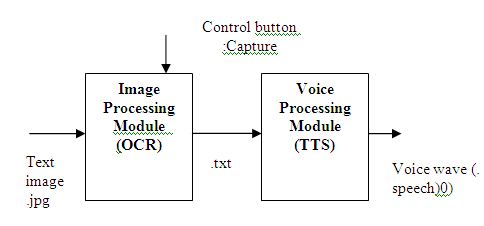
\includegraphics[scale = 1]{img2.png}
    \caption{Block diagram of text-to-speech device.}
    \label{fig:enter-label}
\end{figure}
\vspace{5mm}

\small
Figure 2 shows the block diagram of Text-To-Speech device, 1st block is image processing module, where OCR converts .jpg to .txt form. 2nd is voice processing module which converts .txt to speech. OCR is important element in this module. OCR or Optical Character Recognition is a technology that automatically recognize the character through the optical mechanism, this technology imitate the ability of the human senses of sight, where the camera becomes a replacement for eye and image processing is done in the computer engine as a substitute for the human brain2. Tesseract OCR is a type of OCR engine with matrix matching3. The selection of Tesseract engine is because of its flexibility and extensibility of machines and the fact that many communities are active researchers to develop this OCR engine and also because Tesseract OCR can support 149 languages. In this project we are identifying English alphabets. Before feeding the image to the OCR, it is converted to a binary image to increase the recognition accuracy. Image binary conversion is done by using Imagemagick software, which is another open source tool for image manipulation. The output of OCR is the text, which is stored in a file (speech.txt). Machines still have defects such as distortion at the edges and dim light effect, so it is still difficult for most OCR engines to get high accuracy text4. It needs some supporting and condition in order to get the minimal defect. Tesseract OCR Implementation.

%Salman Johir Tonoy

\textcolor{BlueViolet}
{\subsection{Software Design}}
\small
Software processes the input image and converted into text format. The software implementation is showed in Figure 3.
\vspace{5mm}
\begin{figure}[h]
    \centering
    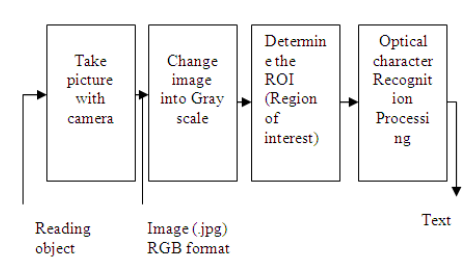
\includegraphics[scale = 1]{img3.png}
    \caption{Software design of image processing module.}
    \label{fig:enter-label}
\end{figure}
\vspace{5mm}

\textcolor{BlueViolet}
{\subsection{The Voice Processing Module}}
\small
In this module text is converted to speech. The out- put of OCR is the text, which is stored in a file (speech. txt). Here, Festival software is used to convert the text to speech. Festival is an open source Text To Speech (TTS) system, which is available in many languages. In this proj- ect, English TTS system is used for reading the text.

\vspace{5mm}
\textcolor{BlueViolet}
{\section{Results}}
Observed outcome of project:\\
\begin{itemize}
    \item Text is extracted from the image and converted to audio.
    \item It recognizes both capital as well as small letters.
    \item It recognizes numbers as well.
    \item Range of reading distance was 38-42cm.
    \item Character font size should be minimum 12pt.
    \item Maximum tilt of the text line is 4-5 degree from the vertical.
\end{itemize}

\textcolor{BlueViolet}
{\section{Conclusion}}
\small
Text-to-Speech device can change the text image input into sound with a performance that is high enough and a readability tolerance of less than 2\%, with the average time processing less than three minutes for A4 paper size. This portable device, does not require internet connection, and can be used independently by people. Through this method, we can make editing process of books or web pages easier.

\textcolor{BlueViolet}
{\section{References}}
\begin{enumerate}
    \item Archana A, Shinde D. Text pre-processing and text seg- mentation for OCR. International Journal of Computer Science Engineering and Technology. 2012:810–12.

    \item Mithe R, Indalkar S, Divekar N. Optical character recog- nition. International Journal of Recent Technology and Engineering. 2013 Mar; 2(1).

    \item Smith R. An overview of the Tesseract OCR engine, USA: Google Inc; 2007.

    \item Shah H, Shah A. Optical character recognition of Gujarati numerical. International Conference on Signals, Systems and Automation. 2009; 49–53.

    \item Monk S. Raspberry pi cook.
    \item Text localization and extraction in images using mathemat- ical morphology and OCR Techniques; 2013.
    \item Vanitha E, Kasarla PK, Kuamarswamy E. Implementation of text- to-speech for real time embedded system using Raspberry Pi processor. International Journal and Magazine of Engineering Technology Management and Research. 2015 Jul:1995.
    \item Kumar GS, Krishna MNVLM. Low cost speech recognition system running on Raspberry Pi to support Automation applications. International Journal of Engineering Trends and Technology. 2015; 21(5).
    \item Bhargava A, Nath KV, Sachdeva P, Samel M. Reading assis- tant for visually Impaired. International Journal of current Engineering and Technology. 2015 Apr; 5(2).

    \item Gomes LCT, Nagle EJ, Chiquito JG. Text-to-speech conver- sion system for Brazilian Portuguese using a formant-based synthesis technique. LPS-DECOM-FEEC-Unicamp.
    
    \item Sim Liew Fong, Abdelrahman Osman Elfaki, Md Gapar bin Md Johar \& Kevin Loo Tow Aik, Mobile Language Translator, 5th Malaysian Conference in Software Engineering (Misses); 2011.
    
    \item Kamesh DBK, Nazma SK, Sastry JKR, Venkateswarlu S. Camera based text to speech conversion, obstacle and cur- rency detection for blind persons. Indian Journal of Science and Technology. 2016 Aug; 9(30).
\end{enumerate}
 



\end{document}
